\documentclass{article}

\usepackage{a4wide}
\usepackage[utf8]{inputenc}
\usepackage[T1]{fontenc}
\usepackage[french]{babel}
\usepackage[babel=true]{csquotes} % guillemets français
\usepackage{graphicx}
\graphicspath{{Images/}}
\usepackage{color}
\usepackage{hyperref}
\hypersetup{colorlinks,linkcolor=,urlcolor=blue}

\usepackage{amsmath}
\usepackage{amssymb}


\title{Rapport}
\author{Kevin Jovien, L3 informatique}
\date{\today}

\begin{document}

\maketitle % pour écrire le titre


%% Le résumé:
\begin{abstract}
  Le présent rapport porte sur la gestion des threads. Pour cela nous allons programmer un mini-jeux de balle. Le jeu possède un tableau des scores qui permet de savoir le temps écoulé et le score, un écran principal qui est tout simplement le jeu et enfin une zone d’interaction avec le jeu . un bouton pause, un bouton qui permet d’ajouter des balles et un qui permet de le retirer. Le tableau des scores et la zone de jeux seront géré par deux threads distincts, pour permettre de gérer aisément la pause simultanée du jeu et de l’horloge. 
\end{abstract}
\section{Introduction}
\label{section:intro} % pour faire référence à la section ailleurs (\ref{...} voir plus bas)

Dans un premier temps on verra le cheminement de la mise en place de l’architecture. Ensuite on verra cette architecture plus en détail et on regardera certains points importants. Puis on soulèvera les points difficiles et les problèmes rencontrent sur le projet. Pour finir, on conclura par une énumération des pistes possibles pour améliorer le programme actuel.

\section{Mise en place de l'architecture}
\label{section:corps} % pour faire référence à la section ailleurs (\ref{...} voir plus bas)

Le jeu ci-dessous peut être séparé en 3 parties.
\begin{center}
  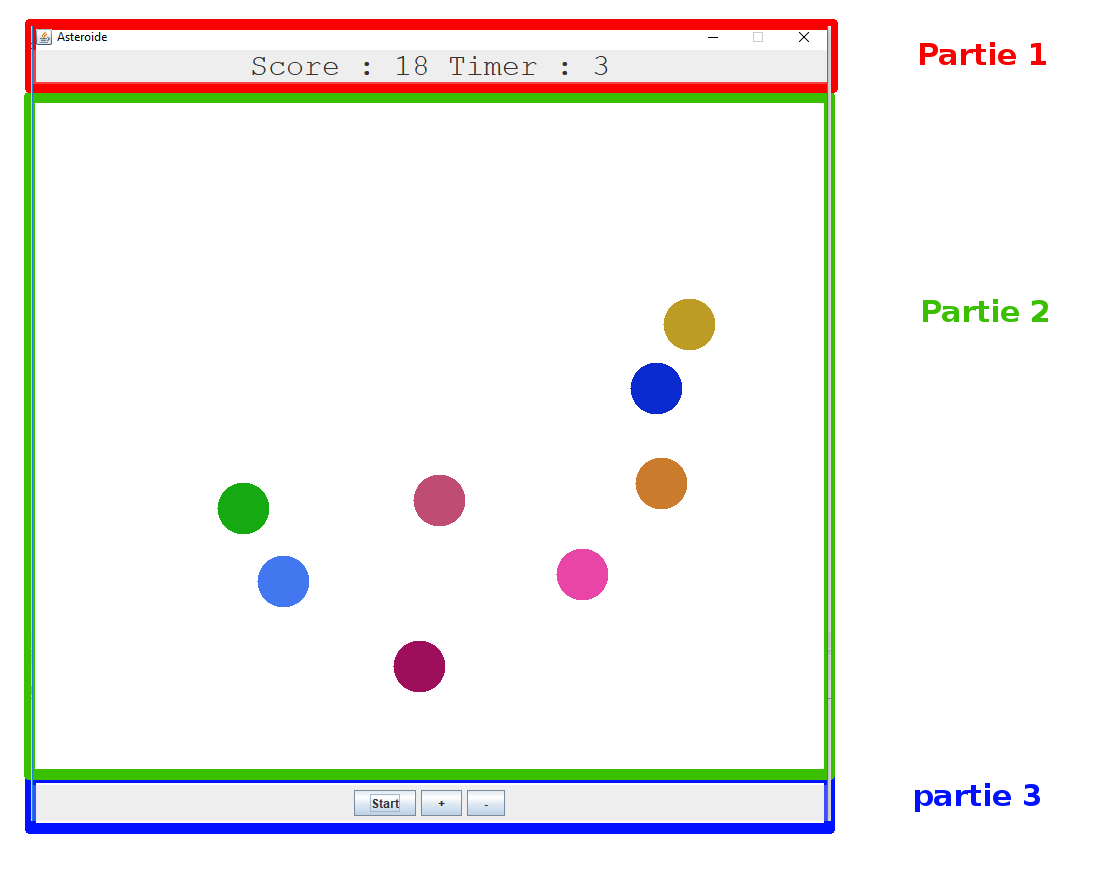
\includegraphics[scale=0.30]{ecranjeu.png}
\end{center}
La première et seconde partie du jeu affichent le tableau des scores et le jeu. Ces zones fonctionnent de la même façon qu’un ordinateur. C'est-à-dire un écran qui va n'être que là pour affiche, on va modéliser cela par une classe « JLabel pour le tableau des scores et un « JPanel » pour l’écran de jeu. Et le centre de calcul (processeur, carte-mère, …) qu’on va ici modéliser par deux threads : une pour le jeu et une pour l’horloge.
\begin{center}
  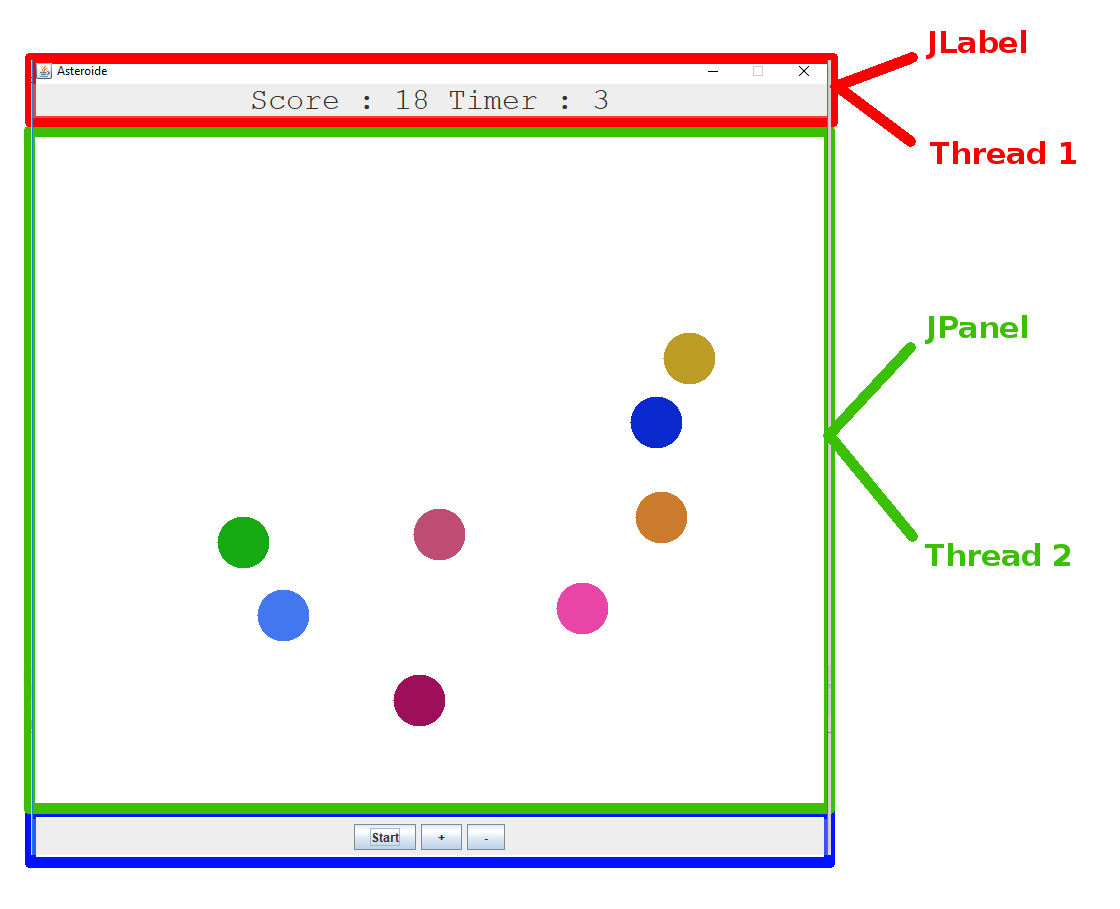
\includegraphics[scale=0.30]{ecranjeu2.png}
\end{center}
L’emploie des deux threads permettra l’implémentation de la fonction pause plus facilement grâce à la méthode \textit{wait()}~\cite{waitDoc}.

\section{Achitecture et Code}
\label{section:hello} % pour faire référence à la section ailleurs (\ref{...} voir plus bas)

On va voir maintenant l'architecture du projet et on va expliquer les méthodes utilisées.

\begin{center}
  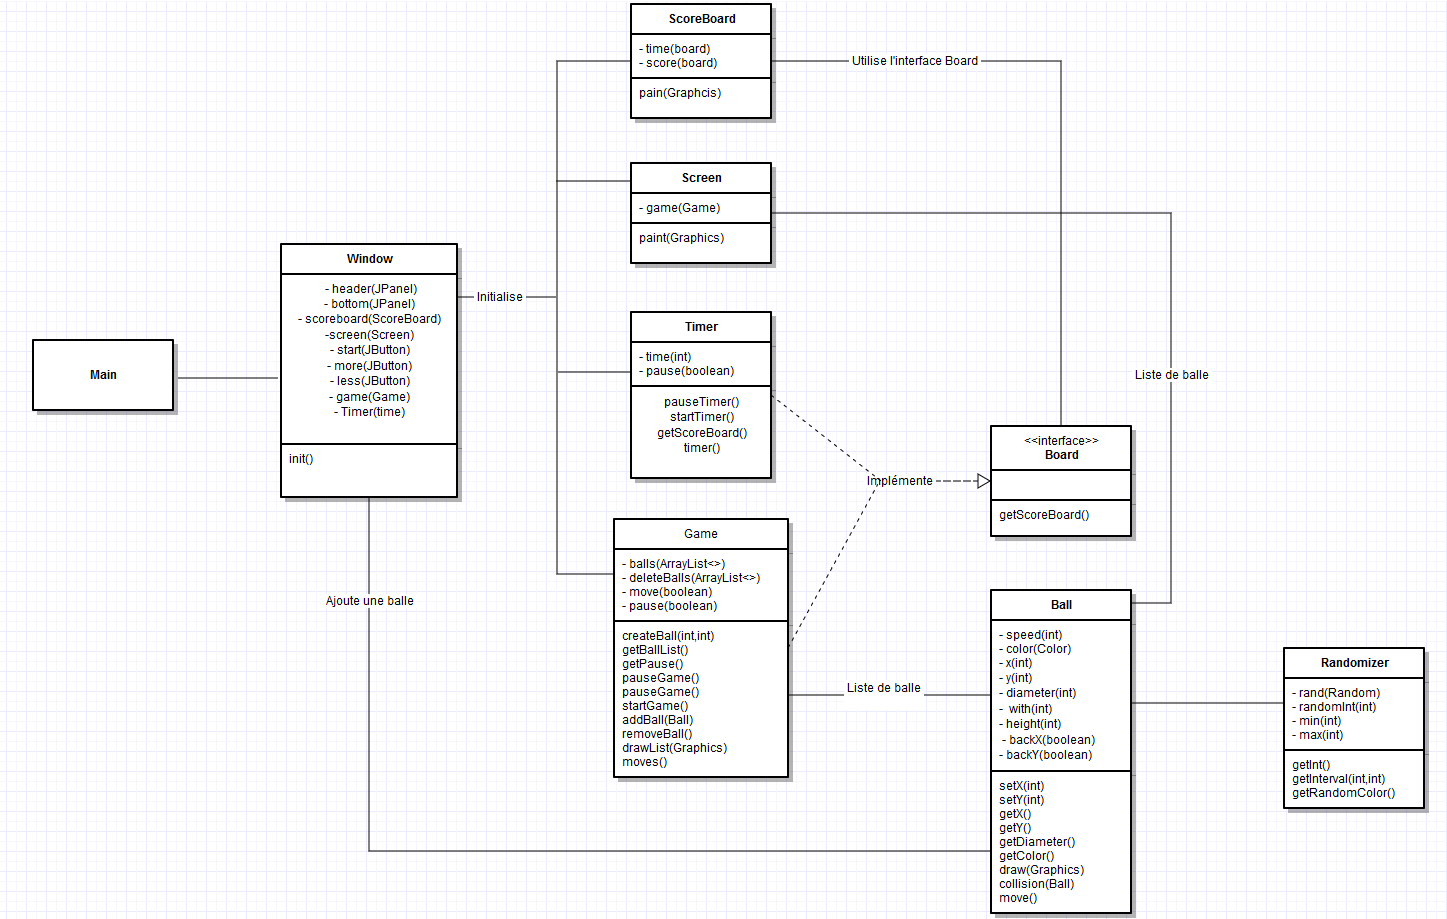
\includegraphics[scale=0.35]{architecture.png}
\end{center}

\subsection{Tableau des scores}
Sur le graphe ci-dessus, « l’architecture du projet », on peut voir que les 2 threads Timer et Game implémente l’interface Board. On a créé cette interface pour faciliter l’utilisation du Jlabel Scoreboard. Elle permet de ne pas ce soucier de l’ordre des arguments et facilite l’affichage des résultats. On appelle \textit{repaint}~\cite{repaintDoc} dans la fonction paint pour permettre un rafraîchissement de la Jlabel grâce à la récursivité. 
\begin{verbatim}
public class ScoreBoard extends JLabel{
    Board score,time;
    public ScoreBoard (Board score,Board time) {
        this.score = score;
        this.time = time;
        this.setFont(new Font("Courier New",Font.LAYOUT_NO_LIMIT_CONTEXT,30));
        this.setText(score.getScoreBoard()+" "+time.getScoreBoard());
        this.setHorizontalAlignment(CENTER);
    }
	
    public void paint(Graphics g) {
        this.setText(score.getScoreBoard()+" "+time.getScoreBoard());
        super.paint(g);
        repaint();
    }
}
\end{verbatim}

\subsection{Le jeu}

\subsubsection{Thread Game}
C’est dans le thread Game qu’on va gérer la ressource critique, la liste de balles. La liste est manipulée par les méthodes move et drawListe(Graphics). On va donc synchroniser ces méthodes car elle accède à la ressource critique « «liste desballes ». On évite ainsi de parcourir la liste lorsque la fonction move est en train de la modifier (suppression, ajout, etc).
Pour rendre l’animation plus naturel, j’ai choisi d’alterner les phases de calcule (ie. les movements de balle) et les phases d’affichages. Pour cela on va utiliser une variable booléen moveball.
\textit{verbatim}:
\begin{verbatim}
    public synchronized void drawList(Graphics g) {
		
        if(!move) {
               for(Ball ball: balls) {
                 ball.draw(g);
               }
              move = true;
        }
    }
	
     public synchronized void moves() {
		
         if(move) {
            try {
              while(pause) {wait();}
            } catch (InterruptedException e1) {
              e1.printStackTrace();
            }
            for(int i = 0 ;i<balls.size();i++) {
                balls.get(i).move();
                for(int j = i+1;j<balls.size();j++ ) {
                   if(balls.get(i).collision(balls.get(j))) {
                        deleteBalls.add(balls.get(i));
                        deleteBalls.add(balls.get(j));
                        score = score + 2;
                   }
                }
            }
            for(Ball delete:deleteBalls) {
               balls.remove(delete);
            }
\end{verbatim}
\subsubsection{Le bouton Pause}
Pour gérer la pause du jeu et de l’horloge, on va utilise la fonction wait() des threads. Pour cela on utilise une variable booléen pour entrer dans une boucle « tant que » et attendre avec wait. L’utilisation de la boucle est importante car il est possible que le thread mis en attente quitte la file. Pour sortir de la file d’attente on va notifier chaque thread avec notify(). On va les placer dans un bloc synchronisé pour permettre leurs utilisations car la fonction notify ne peut utiliser en dehors d’un bloc synchronisé. Et ainsi permettre de sortir de la pause.

\begin{verbatim}
		    start.addActionListener(new ActionListener(){
			        public void actionPerformed(ActionEvent e){
			        	if(!game.getPause()) {
			        		game.pauseGame();
			        		time.pauseTimer();
			        		start.setText("Start");
			        	}else {
			        		game.startGame();
			        		time.startTimer();
			        		synchronized (time) {
			        			time.notify();
							}
			        		synchronized (game) {
								game.notify();
							}
			        		start.setText("Stop");

			        	}
			        }
		        });
\end{verbatim}

\subsection{Problème rencontre et difficultés}
L’une des difficultés rencontre a été de savoir quels éléments devrait être gérée par un thread et déterminer la variable critique commune. J’ai donc décidé que l'élément critique serait manipulé que par le thread Game car pour moi la seule variable critique était la liste de balles. Un autre problème rencontré était la gestion de la fonction wait. Car l’utilisation de la fonction notifyall provoque un bug du thread Timer. Pour corriger le bug j’ai donc utilisé un simple \textit{notify}~\cite{notifyDoc} pour cibler le thread important. 

\subsection{Conclusion}
Pour améliorer le jeu, on pourrait ajouter quelques fonctionnalités supplémentaires comme des effets sonores en utilisant  un AudioInputStream au moment des collisions entre les balles et les murs. Ou encore permettre aux joueurs de déplacer les balles après une pause aléatoire en utilisant l’event mouse click sur le Jpanel Screen. 
%%% La bibliographie:
\bibliographystyle{plain}
\bibliography{ma_biblio}

\end{document}
